\documentclass[journal,12pt,twocolumn]{IEEEtran}
\usepackage{setspace}
\usepackage{gensymb}
\usepackage{iithtlc}
%\usepackage{xcolor}
\usepackage{caption}
\usepackage{fullpage}
\usepackage[american]{circuitikz}
\usetikzlibrary{circuits.logic.US}
\usepackage{circuitikz}
\usetikzlibrary{positioning}
\usetikzlibrary{matrix,calc}
%\usepackage{subcaption}
%\doublespacing
\singlespacing

%\usepackage{graphicx}
%\usepackage{amssymb}
%\usepackage{relsize}
\usepackage[cmex10]{amsmath}
\usepackage{mathtools}
%\usepackage{amsthm}
%\interdisplaylinepenalty=2500
%\savesymbol{iint}
%\usepackage{txfonts}
%\restoresymbol{TXF}{iint}
%\usepackage{wasysym}
\usepackage{amsthm}
\usepackage{mathrsfs}
\usepackage{txfonts}
\usepackage{stfloats}
\usepackage{cite}
\usepackage{cases}
\usepackage{subfig}
%\usepackage{xtab}
\usepackage{longtable}
\usepackage{multirow}
%\usepackage{algorithm}
%\usepackage{algpseudocode}
\usepackage{enumitem}
\usepackage{mathtools}

\usepackage[framemethod=tikz]{mdframed}

%\usepackage{listings}
%\usepackage{listings}
%    \usepackage[latin1]{inputenc}                                 %%
%    \usepackage{color}                                            %%
%    \usepackage{array}                                            %%
%    \usepackage{longtable}                                        %%
%    \usepackage{calc}                                             %%
%    \usepackage{multirow}                                         %%
    \usepackage{hhline}                                           %%
    \usepackage{ifthen}                                           %%
  %optionally (for landscape tables embedded in another document): %%
    \usepackage{lscape}     
\usepackage{tikz}


%\usepackage{stmaryrd}


%\usepackage{wasysym}
%\newcounter{MYtempeqncnt}
\DeclareMathOperator*{\Res}{Res}
%\renewcommand{\baselinestretch}{2}
\renewcommand\thesection{\arabic{section}}
\renewcommand\thesubsection{\thesection.\arabic{subsection}}
\renewcommand\thesubsubsection{\thesubsection.\arabic{subsubsection}}

\renewcommand\thesectiondis{\arabic{section}}
\renewcommand\thesubsectiondis{\thesectiondis.\arabic{subsection}}
\renewcommand\thesubsubsectiondis{\thesubsectiondis.\arabic{subsubsection}}

% correct bad hyphenation here
\hyphenation{op-tical net-works semi-conduc-tor}

%\lstset{
%language=C,
%frame=single, 
%breaklines=true
%}

%\lstset{
	%%basicstyle=\small\ttfamily\bfseries,
	%%numberstyle=\small\ttfamily,
	%language=Octave,
	%backgroundcolor=\color{white},
	%%frame=single,
	%%keywordstyle=\bfseries,
	%%breaklines=true,
	%%showstringspaces=false,
	%%xleftmargin=-10mm,
	%%aboveskip=-1mm,
	%%belowskip=0mm
%}

%\surroundwithmdframed[width=\columnwidth]{lstlisting}
%\def\inputGnumericTable{}                                 %%

%\lstset{
%language=C,
%frame=single, 
%breaklines=true
%}
%\lstset{
%language=assembly,
%frame=single, 
%breaklines=true
%}
 

\begin{document}
%

\theoremstyle{definition}
\newtheorem{theorem}{Theorem}[section]
\newtheorem{problem}{Problem}
\newtheorem{proposition}{Proposition}[section]
\newtheorem{lemma}{Lemma}[section]
\newtheorem{corollary}[theorem]{Corollary}
\newtheorem{example}{Example}[section]
\newtheorem{definition}{Definition}[section]
%\newtheorem{algorithm}{Algorithm}[section]
%\newtheorem{cor}{Corollary}
\newcommand{\BEQA}{\begin{eqnarray}}
\newcommand{\EEQA}{\end{eqnarray}}
\newcommand{\define}{\stackrel{\triangle}{=}}

\bibliographystyle{IEEEtran}
%\bibliographystyle{ieeetr}

\providecommand{\nCr}[2]{\,^{#1}C_{#2}} % nCr
\providecommand{\nPr}[2]{\,^{#1}P_{#2}} % nPr
\providecommand{\mbf}{\mathbf}
\providecommand{\pr}[1]{\ensuremath{\Pr\left(#1\right)}}
\providecommand{\qfunc}[1]{\ensuremath{Q\left(#1\right)}}
\providecommand{\sbrak}[1]{\ensuremath{{}\left[#1\right]}}
\providecommand{\lsbrak}[1]{\ensuremath{{}\left[#1\right.}}
\providecommand{\rsbrak}[1]{\ensuremath{{}\left.#1\right]}}
\providecommand{\brak}[1]{\ensuremath{\left(#1\right)}}
\providecommand{\lbrak}[1]{\ensuremath{\left(#1\right.}}
\providecommand{\rbrak}[1]{\ensuremath{\left.#1\right)}}
\providecommand{\cbrak}[1]{\ensuremath{\left\{#1\right\}}}
\providecommand{\lcbrak}[1]{\ensuremath{\left\{#1\right.}}
\providecommand{\rcbrak}[1]{\ensuremath{\left.#1\right\}}}
\theoremstyle{remark}
\newtheorem{rem}{Remark}
\newcommand{\sgn}{\mathop{\mathrm{sgn}}}
\providecommand{\abs}[1]{\left\vert#1\right\vert}
\providecommand{\res}[1]{\Res\displaylimits_{#1}} 
\providecommand{\norm}[1]{\lVert#1\rVert}
\providecommand{\mtx}[1]{\mathbf{#1}}
\providecommand{\mean}[1]{E\left[ #1 \right]}
\providecommand{\fourier}{\overset{\mathcal{F}}{ \rightleftharpoons}}
%\providecommand{\hilbert}{\overset{\mathcal{H}}{ \rightleftharpoons}}
\providecommand{\system}{\overset{\mathcal{H}}{ \longleftrightarrow}}
	%\newcommand{\solution}[2]{\textbf{Solution:}{#1}}
\newcommand{\solution}{\noindent \textbf{Solution: }}
\providecommand{\dec}[2]{\ensuremath{\overset{#1}{\underset{#2}{\gtrless}}}}
%\numberwithin{equation}{subsection}
\numberwithin{equation}{problem}
%\numberwithin{problem}{subsection}
%\numberwithin{definition}{subsection}
%\makeatletter
%\@addtoreset{figure}{problem}
%\makeatother
%
%\let\StandardTheFigure\thefigure
%%\renewcommand{\thefigure}{\theproblem.\arabic{figure}}
%\renewcommand{\thefigure}{\theproblem}
%

%\numberwithin{figure}{subsection}

%\numberwithin{equation}{subsection}
%\numberwithin{equation}{section}
%%\numberwithin{equation}{problem}
%%\numberwithin{problem}{subsection}
\numberwithin{problem}{section}
%%\numberwithin{definition}{subsection}
%\makeatletter
%\@addtoreset{figure}{problem}
%\makeatother
\makeatletter
\@addtoreset{table}{problem}
\makeatother

\let\StandardTheFigure\thefigure
\let\StandardTheTable\thetable
%%\renewcommand{\thefigure}{\theproblem.\arabic{figure}}
%\renewcommand{\thefigure}{\theproblem}
\renewcommand{\thetable}{\theproblem}
%%\numberwithin{figure}{section}

%%\numberwithin{figure}{subsection}

\renewcommand{\thefigure}{\theenumi}

\def\putbox#1#2#3{\makebox[0in][l]{\makebox[#1][l]{}\raisebox{\baselineskip}[0in][0in]{\raisebox{#2}[0in][0in]{#3}}}}
     \def\rightbox#1{\makebox[0in][r]{#1}}
     \def\centbox#1{\makebox[0in]{#1}}
     \def\topbox#1{\raisebox{-\baselineskip}[0in][0in]{#1}}
     \def\midbox#1{\raisebox{-0.5\baselineskip}[0in][0in]{#1}}

\vspace{3cm}

\title{ 
	\logo{
GATE Exercises on Boolean Logic 
	}
}



% paper title
% can use linebreaks \\ within to get better formatting as desired
%\title{Matrix Analysis through Octave}
%
%
% author names and IEEE memberships
% note positions of commas and nonbreaking spaces ( ~ ) LaTeX will not break
% a structure at a ~ so this keeps an author's name from being broken across
% two lines.
% use \thanks{} to gain access to the first footnote area
% a separate \thanks must be used for each paragraph as LaTeX2e's \thanks
% was not built to handle multiple paragraphs
%

%\author{G V V Sharma$^{*}$% <-this % stops a space
%\thanks{*The author is with the Department
%of Electrical Engineering, Indian Institute of Technology, Hyderabad
%502285 India e-mail:  gadepall@iith.ac.in.}% <-this % stops a space
%%\thanks{J. Doe and J. Doe are with Anonymous University.}% <-this % stops a space
%%\thanks{Manuscript received April 19, 2005; revised January 11, 2007.}}
%}
% note the % following the last \IEEEmembership and also \thanks - 
% these prevent an unwanted space from occurring between the last author name
% and the end of the author line. i.e., if you had this:
% 
% \author{....lastname \thanks{...} \thanks{...} }
%                     ^------------^------------^----Do not want these spaces!
%
% a space would be appended to the last name and could cause every name on that
% line to be shifted left slightly. This is one of those "LaTeX things". For
% instance, "\textbf{A} \textbf{B}" will typeset as "A B" not "AB". To get
% "AB" then you have to do: "\textbf{A}\textbf{B}"
% \thanks is no different in this regard, so shield the last } of each \thanks
% that ends a line with a % and do not let a space in before the next \thanks.
% Spaces after \IEEEmembership other than the last one are OK (and needed) as
% you are supposed to have spaces between the names. For what it is worth,
% this is a minor point as most people would not even notice if the said evil
% space somehow managed to creep in.



% The paper headers
%\markboth{Journal of \LaTeX\ Class Files,~Vol.~6, No.~1, January~2007}%
%{Shell \MakeLowercase{\textit{et al.}}: Bare Demo of IEEEtran.cls for Journals}
% The only time the second header will appear is for the odd numbered pages
% after the title page when using the twoside option.
% 
% *** Note that you probably will NOT want to include the author's ***
% *** name in the headers of peer review papers.                   ***
% You can use \ifCLASSOPTIONpeerreview for conditional compilation here if
% you desire.




% If you want to put a publisher's ID mark on the page you can do it like
% this:
%\IEEEpubid{0000--0000/00\$00.00~\copyright~2007 IEEE}
% Remember, if you use this you must call \IEEEpubidadjcol in the second
% column for its text to clear the IEEEpubid mark.



% make the title area
\maketitle

%\tableofcontents

\bigskip

\begin{abstract}
%\boldmath
This problem set has questions related to Boolean logic and gates taken from GATE papers over the last twenty years.  Teachers can use the problem set for courses tutorials. 
 
\end{abstract}

\begin{enumerate}
\item The Boolean expression$(X+Y)(X+\overline{Y})+(\overline{X\overline{Y})+\overline{X}}$ simplifies to
      \begin{enumerate}
      \item X
      \item Y
      \item XY
      \item X+Y
      \end{enumerate}
 
\item The SOP (sum of products) form of a Boolean function is$\sum(0,1,3,7,11)$,where inputs are A,B,C,D(A is MSB,and D is LSB).The equivalent minimised expression of the function is  
      \begin{enumerate}
      \item $(\overline{B}+C)(\overline{A}+C)(\overline{A}+\overline{B})(\overline{C}+D)$
      \item $(\overline{B}+C)(\overline{A}+C)(\overline{A}+\overline{C})(\overline{C}+D)$
      \item $(\overline{B}+C)(\overline{A}+C)(\overline{A}+\overline{C})(\overline{C}+\overline{D})$
      \item $(\overline{B}+C)(A+\overline{B})(\overline{A}+\overline{B})(\overline{C}+D)$
      \end{enumerate}
\item The Boolean expression$F(X,Y,Z)=\overline{X}Y\overline{Z}+X\overline{Y}.\overline{Z}+XY\overline{Z}+XYZ $ converted into the canonical product of sum (POS) form is
      \begin{enumerate}
      \item $(X+Y+Z)(X+Y+\overline{Z})(X+Y+\overline{Z})(X+\overline{Y}+\overline{Z})(\overline{X}+Y+\overline{Z})$
      \item $(X+\overline{Y}+Z)(\overline{X}+Y+Z)(\overline{X}+\overline{Y}+Z)(\overline{X}+\overline{Y}+\overline{Z})$
      \item $(X+Y+Z)(\overline{X}+Y+\overline{Z})(X+\overline{Y}+Z)$
      \item $(X+\overline{Y}+\overline{Y})(\overline{X}+Y+Z)(X+Y+Z)$
      \end{enumerate}
\item If the functions W, X, Y and Z are as follows $W=R+\overline{P}Q+\overline{R}S$
$X=PQ\overline{R}.\overline{S}+\overline{P}.\overline{Q}.\overline{R}.
\overline{S}+P\overline{Q}.\overline{R}.\overline{S}$ $Y=RS+\overline{PR+P\overline{Q}+\overline{P}.\overline{Q}}$ $Z=R+S+\overline{PQ+\overline{P}.\overline{Q}.\overline{R}+P\overline{Q}.\overline{S}}$
     \begin{enumerate}
      \item $W = Z, X =\overline{Z}$ 
      \item W = Z, X = Y
      \item W=Y
      \item W = $Y =\overline{Z}$
     \end{enumerate}
\item The Boolean expression $AC +B\overline{C}$ is equivalent to
     \begin{enumerate}
      \item $AC+\overline{BC}$ 
      \item $\overline{B}C+AC+B\overline{C}+\overline{A}C\overline{B}$
      \item $AC+B\overline{C}+\overline{B}C+ABC$
      \item $ABC+A\overline{B}.C+AB\overline{C}+\overline{A}.B.\overline{C}$
    \end{enumerate}
    \item The boolean expression $Y=\overline{A}.\overline{B}.\overline{C}D+\overline{A}BC\overline{D}+A\overline{B}.\overline{C}
D+AB\overline{C}.\overline{D}$ can be
\begin{enumerate} 
      \item $Y=\overline{A}.\overline{B}.\overline{C}D+\overline{A}B\overline{C}+A\overline{C}D$
      \item $Y=\overline{A}.\overline{B}.\overline{C}D+BC\overline{D}+A\overline{B}.\overline{C}D$
      \item $Y=\overline{A}BC\overline{D}+\overline{B}.\overline{C}D+
A\overline{B}.\overline{C}D$
      \item $Y=\overline{A}BC\overline{D}+\overline{B}.\overline{C}D+
AB\overline{C}.\overline{D}$
    \end{enumerate}
 \item The Boolean expression$ \overline{X}Y\overline{Z}+\overline{X}.\overline{Y}Z+XY\overline{Z}
+X\overline{Y}Z+XYZ$ cab be simplified to
\begin{enumerate}
      \item $X\overline{Z}+\overline{X}Z+YZ$
      \item $XZ+\overline{Y}Z+Y\overline{Z}$
      \item $\overline{X}Y+YZ+XZ$
      \item $\overline{X}\overline{Y}+Y\overline{Z}+\overline{X}Z$
    \end{enumerate}
\item The simplified form of the Boolean expression $Y=(\overline{A}BC+D)(\overline{A}D+\overline{B}.\overline{C})$ can be written as
   \begin{enumerate}
      \item $\overline{A}D+\overline{B}.\overline{C}D$
      \item $AD+B\overline{C}D$
      \item $(\overline{A}+D)(\overline{B}C+\overline{D})$
      \item $A\overline{D}+BC\overline{D}$
    \end{enumerate}
\item A function of Boolean variables X, Y and Z is expressed in terms of the min-terms as $$F(X,Y,Z)=\sum(1,2,5,6,7)$$ Which one of the product of sums given below is equal to the function F(X,Y,Z)?
    \begin{enumerate}
      \item $(\overline{X}+\overline{Y}+\overline{Z})(\overline{X}+Y+Z)(X+\overline{Y}+\overline{Z})$
      \item $(X+Y+Z)(X+\overline{Y}+\overline{Z})(\overline{X}+Y+Z)$
      \item $(\overline{X}+\overline{Y}+Z)(\overline{X}+Y+\overline{Z}(X+\overline{Y}+Z)(X+Y+\overline{Z})(X+Y+Z)$
      \item $(X+Y+\overline{Z})(\overline{X}+Y+Z)(\overline{X}+Y+\overline{Z})(\overline{X}+\overline{Y}+Z)(\overline{X}+\overline{Y}+\overline{Z})$
    \end{enumerate}

\item For the logic circuit shown in Fig., the required input condition (A,B,C) to
make the output (X)=1 is
%
\begin{figure}[!h]
\centering
\resizebox {\columnwidth} {!} {
%\documentclass[tikz,border=2mm]{standalone}
%\usetikzlibrary{circuits.logic.US}

%\begin{document}
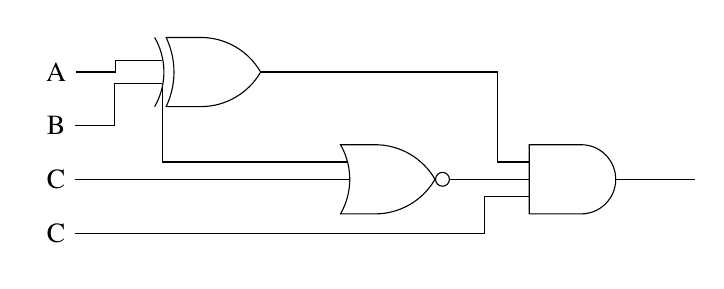
\begin{tikzpicture}[circuit logic US, huge circuit symbols]
  \matrix[column sep=10mm]
    {
      \node (a) {A}; & \node [xor gate] (nand) {};&& \\
      \node (b) {B}; &&& \\
      \node (c) {C}; && \node [nor gate, inputs=nnn] (nor) {}; & \node [and gate, inputs=nnn] (out) {}; \\
                     
      \node (d) {C};&&& \\
    };
    \draw (a.east) -- ++(right:5mm)       |- (nand.input 1);
    \draw (b.east) -- ++(right:5mm)       |- (nand.input 2);
    \draw (c.east) -- ++(right:5mm)       |- (nor.input 2);
    \draw (d.east) -- ++(right:52mm)      |- (out.input 3);
    
  
    \draw (nand.output) -- ++(right:30mm) |- (out.input 1);
    \draw (nand.input 2)  |- (nor.input 1);
    \draw (nor.output) -- ++(right:5mm)   |- (out.input 2);
    \draw (out.output) -- ++(right:10mm);
\end{tikzpicture}
%\end{document}

}
\caption{}
%\label{fig:$10$}
\end{figure}
%
    
%                         \begin{figure}[!h]
%                         \centering
%                         \includegraphics[width=\columnwidth]{./figs/figure1.eps}
%						\captionof{figure}{}
%						\label{fig:1}
%                         \end{figure}  
     \begin{enumerate}
      \item $ 1,0,1$
      \item $0,0,1$
      \item $1,1,1$
      \item $0,1,1$
    \end{enumerate}
   
    
    \item For the logic circuit shown in Fig., the simplified Boolean expression for the
output Y is
\begin{figure}[!h]
\centering
\resizebox {\columnwidth} {!} {
%\documentclass{article}

%\usepackage{circuitikz}

%\begin{document}

\begin{circuitikz} \draw
 
 

  (0,5) node[nand port] (mygate) {}
  (-1.2,4.72) to [short,-*] (-1.2,4.72)
  (-2,6) node[nand port] (myand3) {}
  (myand3.in 1) node[anchor=east] {$A$}
  (myand3.in 2) node[anchor=east] {$B$}
  
 
  (3,4) node[nand port] (myand1) {}
  
  (1.7,3.7) to [short,-*] (1.77,3.7)

 
  (3,2) node[nor port] (myand2) {}
  (myand2.in 2) -- +(-5,0)
  (myand2.in 2) node[anchor=east] {$C$}
  
  (1.9,1.7) to [short,-*] (2,1.7)
   (mygate.out) -| (myand1.in 1)
  (0.16,5) to [short,-*] (.18,5)
  (mygate.out) |- (myand2.in 1) 
  (5,3) node[nor port] (myor) {}
  (myor.out) node[anchor=west] {$Y$}
  (myand1.out) |- (myor.in 1)
  (myand2.out) |- (myor.in 2)
  (myand3)-| (mygate.in 1)
  (mygate.in 2)|- (myand1.in 2)
  (mygate.in 2) -|(myand3.in 2)
  
  
;\end{circuitikz}

%\end{document}

}
\caption{}
%\label{fig:$10$}
\end{figure}

%\begin{figure}[!h]
%\centering
%\resizebox {\columnwidth} {!} {
%%\documentclass{article}

%\usepackage{circuitikz}

%\begin{document}

\begin{circuitikz} \draw
 
 

  (0,5) node[nand port] (mygate) {}
  (-1.2,4.72) to [short,-*] (-1.2,4.72)
  (-2,6) node[nand port] (myand3) {}
  (myand3.in 1) node[anchor=east] {$A$}
  (myand3.in 2) node[anchor=east] {$B$}
  
 
  (3,4) node[nand port] (myand1) {}
  
  (1.7,3.7) to [short,-*] (1.77,3.7)

 
  (3,2) node[nor port] (myand2) {}
  (myand2.in 2) -- +(-5,0)
  (myand2.in 2) node[anchor=east] {$C$}
  
  (1.9,1.7) to [short,-*] (2,1.7)
   (mygate.out) -| (myand1.in 1)
  (0.16,5) to [short,-*] (.18,5)
  (mygate.out) |- (myand2.in 1) 
  (5,3) node[nor port] (myor) {}
  (myor.out) node[anchor=west] {$Y$}
  (myand1.out) |- (myor.in 1)
  (myand2.out) |- (myor.in 2)
  (myand3)-| (mygate.in 1)
  (mygate.in 2)|- (myand1.in 2)
  (mygate.in 2) -|(myand3.in 2)
  
  
;\end{circuitikz}

%\end{document}

%}
%\caption{}
%\label{fig:problem11}
%\end{figure}

   \begin{enumerate}
     \item A+B+C
      \item 0
      \item 1
      \item C
    \end{enumerate} 
    
     \item If X=1 in logic equation $[X+Z{\overline{Y}+(\overline{Z}+X\overline{Y})}]{\overline{X}+\overline{Z}(X+Y)}=1,$ then
    \begin{enumerate}
      \item Y=Z
      \item $Y=\overline{Z}$
      \item $Z=1$
      \item $Z=0$
    \end{enumerate}
     \item The output Y in the circuit below is always '1' when
\begin{figure}[!h]
\centering
\resizebox {\columnwidth} {!} {
%\documentclass{article}
%\usepackage{circuitikz}

%\begin{document}

\begin{circuitikz} 
\draw
  (2,3) node[nand port] (nand6) {}
  (0,4) node[nand port] (nand5) {}
  (0,2.5) node[nand port] (nand4) {}
  (4,3) node[nand port] (nand3) {}
  (6,2) node[nand port] (nand2) {}
  (nand2.out) node[anchor=west] {$Y$}
  (0,1) node[nand port] (nand1) {}
  (nand1.out) -| (nand2.in 2)
 
  (nand3.out) -| (nand2.in 1)
  (nand3.in 1) -| (nand3.in 2)
  (nand6.out) -| (nand3.in 2)
  (nand4.out) -| (nand6.in 2)
  (nand5.out) -| (nand6.in 1)
  (nand5.in 2) -| (nand4.in 1)
  (nand4.in 2) -| (nand1.in 1)
  
  ;
\draw 
    ([xshift=-1cm]nand1.in 1) 
      coordinate (aux) node[left] {$R$} to[short] 
    (nand1.in 1);
\draw 
    ([xshift=-1cm]nand1.in 2) 
        node[left] {$P$} to[short] 
    (nand1.in 2);

\draw 
    ([xshift=-1cm]nand5.in 1) 
        node[left] {$P$} to[short]
    (nand5.in 1);

\draw 
    ([xshift=-1cm]nand4.in 1) 
        node[left] {$Q$} to[short]
    (nand4.in 1);



\end{circuitikz}

%\end{document}
}
\caption{}
%\label{fig:$10$}
\end{figure}

%
     
%                         \begin{figure}[!h]
%                         \centering
%                         \includegraphics[width=\columnwidth]{./figs/problem16.tex}
%                         \captionof{figure}{}
%                         \label{fig:4}
%                         \end{figure}  
  
   \begin{enumerate}
      \item two or more of the inputs P,Q,R are '0'
      \item two or more of the inputs P,Q,R are '1'
      \item any odd number of the inputs P,Q,R is '0'
      \item any odd number of the inputs P,Q,R is '1'
    \end{enumerate} 
    \item In the sum of product function f(X,Y,Z)=$\sum(2,3,4,5)$,prime implicants are
    \begin{enumerate}
      \item $\overline{X}Y,X\overline{Y}$
      \item $\overline{X}Y,X\overline{Y}.\overline{Z},X\overline{Y}Z$
      \item $\overline{X}Y\overline{Z},\overline{X}YZ,X\overline{Y}$
      \item $\overline{X}Y\overline{Z},\overline{X}YZ,X\overline{Y}.\overline{Z},X\overline{Y}Z$
    \end{enumerate}
    \item The logic function f=$\overline{(X.\overline{Y})+(\overline{X}.Y)}$ is same as
    \begin{enumerate}
      \item $(X+Y)(\overline{X}+\overline{Y})$
      \item $\overline{(\overline{X}+\overline{Y})+(X+Y)}$
      \item $(\overline{XY}).(\overline{X}.\overline{Y})$
      \item None of the above
    \end{enumerate}
    \item The minimal product of sums function described by the K-map given in Fig.
\begin{figure}[!h]
\centering
\resizebox {\columnwidth} {!} {
%\documentclass{standalone}
%\usepackage{tikz}
%\usetikzlibrary{matrix,calc}



%Empty Karnaugh map 2x4
\newenvironment{Karnaughvuit}%
{
\begin{tikzpicture}[baseline=(current bounding box.north),scale=0.8]
\draw (0,0) grid (4,2);
\draw (0,2) -- node [pos=0.7,above right,anchor=south west] {AB} node [pos=0.7,below left,anchor=north east] {C} ++(135:1);
%
\matrix (mapa) [matrix of nodes,
        column sep={0.8cm,between origins},
        row sep={0.8cm,between origins},
        every node/.style={minimum size=0.3mm},
        anchor=4.center,
        ampersand replacement=\&] at (0.5,0.5)
{
                      \& |(c00)| 00         \& |(c01)| 01         \& |(c11)| 11         \& |(c10)| 10         \& |(cf)| \phantom{00} \\
|(r00)| 0             \& |(0)|  \phantom{0} \& |(1)|  \phantom{0} \& |(3)|  \phantom{0} \& |(2)|  \phantom{0} \&                     \\
|(r01)| 1             \& |(4)|  \phantom{0} \& |(5)|  \phantom{0} \& |(7)|  \phantom{0} \& |(6)|  \phantom{0} \&                     \\
|(rf) | \phantom{00}  \&                    \&                    \&                    \&                    \&                     \\
};
}%
{
\end{tikzpicture}
}


%Defines 8 or 16 values (0,1,X)
\newcommand{\contingut}[1]{%
\foreach \x [count=\xi from 0]  in {#1}
     \path (\xi) node {\x};
}



%\begin{document}
    
    %
    \begin{Karnaughvuit}
       \contingut{1,1,0,x,0,0,0,x}
    \end{Karnaughvuit}
    %
    

%\end{document}

}
\captionof{figure}{}
%\label{fig:$10$}
\end{figure}

%\begin{figure}[!h]
%\centering
%\resizebox {\columnwidth} {!} {
%%\documentclass{article}
%\usepackage{circuitikz}

%\begin{document}

\begin{circuitikz} 
\draw
  (0,-0.5) node[nand port] (nand9){}
  (2,0) node [nand port](nand8){}
  (4,0) node[nand port](nand7){}
  (2,3) node[nand port] (nand6) {}
  (0,4) node[nand port] (nand5) {}
  (0,2.5) node[nand port] (nand4) {}
  (4,3) node[nand port] (nand3) {}
  (6,1.5) node[nand port] (nand2) {}
  (nand2.out) node[anchor=west] {$Y$}
  (0,1) node[nand port] (nand1) {}
  (nand1.out) -| (nand8.in 1)
  
  (nand8.out)-|(nand7.in 2)
  (nand7.in 1)-|(nand7.in 2)
  (nand7.out)-|(nand2.in 2)
  (nand3.out) -| (nand2.in 1)
  (nand3.in 1) -| (nand3.in 2)
  (nand6.out) -| (nand3.in 2)
  (nand4.out) -| (nand6.in 2)
  (nand5.out) -| (nand6.in 1)
  (nand5.in 2) -| (nand5.in 1)
  (nand4.in 2)-| (nand4.in 1)
  (nand1.in 2) -|(nand1.in 1)
  (nand9.in 2)-|(nand9.in 1)
  (nand9.out)-|(nand8.in 2)
  ;
\draw 
    ([xshift=-1cm]nand1.in 1) 
      coordinate (aux) node[left] {$R$} to[short] 
    (nand1.in 1);


\draw 
    ([xshift=-1cm]nand5.in 1) 
        node[left] {$P$} to[short]
    (nand5.in 1);

\draw 
    ([xshift=-1cm]nand4.in 1) 
        node[left] {$Q$} to[short]
    (nand4.in 1);
\draw 
    ([xshift=-1cm]nand9.in 1) 
        node[left] {$S$} to[short]
    (nand9.in 1);


\end{circuitikz}

%\end{document}
%}
%\caption{}
%\label{fig:problem17}
%\end{figure}
  
   \begin{enumerate}
      \item $\overline{A}.\overline{C}$
      \item $\overline{A}+\overline{C}$
      \item $A+C$
      \item $AC$
    \end{enumerate}
    \item For the circuit shown in Fig., the Boolean expression for the output Y in terms of inputs P, Q,R and S is
\begin{figure}[!h]
\centering
\resizebox {\columnwidth} {!} {
%\documentclass{article}
%\usepackage{circuitikz}

%\begin{document}

\begin{circuitikz} 
\draw
  (0,-0.5) node[nand port] (nand9){}
  (2,0) node [nand port](nand8){}
  (4,0) node[nand port](nand7){}
  (2,3) node[nand port] (nand6) {}
  (0,4) node[nand port] (nand5) {}
  (0,2.5) node[nand port] (nand4) {}
  (4,3) node[nand port] (nand3) {}
  (6,1.5) node[nand port] (nand2) {}
  (nand2.out) node[anchor=west] {$Y$}
  (0,1) node[nand port] (nand1) {}
  (nand1.out) -| (nand8.in 1)
  
  (nand8.out)-|(nand7.in 2)
  (nand7.in 1)-|(nand7.in 2)
  (nand7.out)-|(nand2.in 2)
  (nand3.out) -| (nand2.in 1)
  (nand3.in 1) -| (nand3.in 2)
  (nand6.out) -| (nand3.in 2)
  (nand4.out) -| (nand6.in 2)
  (nand5.out) -| (nand6.in 1)
  (nand5.in 2) -| (nand5.in 1)
  (nand4.in 2)-| (nand4.in 1)
  (nand1.in 2) -|(nand1.in 1)
  (nand9.in 2)-|(nand9.in 1)
  (nand9.out)-|(nand8.in 2)
  ;
\draw 
    ([xshift=-1cm]nand1.in 1) 
      coordinate (aux) node[left] {$R$} to[short] 
    (nand1.in 1);


\draw 
    ([xshift=-1cm]nand5.in 1) 
        node[left] {$P$} to[short]
    (nand5.in 1);

\draw 
    ([xshift=-1cm]nand4.in 1) 
        node[left] {$Q$} to[short]
    (nand4.in 1);
\draw 
    ([xshift=-1cm]nand9.in 1) 
        node[left] {$S$} to[short]
    (nand9.in 1);


\end{circuitikz}

%\end{document}
}
\caption{}
%\label{fig:problem18}
\end{figure}
      \begin{enumerate}
      \item $\overline{P}+\overline{Q}+\overline{R}+\overline{S}$
      \item $P+Q+R+S$
      \item $(\overline{P}+\overline{Q})(\overline{R}+\overline{S})$
      \item $(P+Q)(R+S)$
    \end{enumerate}
    \item The following Karnaugh map represents a function F(X,Y,Z),minimized form of the function F is
\begin{figure}[!h]
\centering
\resizebox {\columnwidth} {!} {
%\documentclass{standalone}
%\usepackage{tikz}
\usetikzlibrary{matrix,calc}



%Empty Karnaugh map 2x4
\newenvironment{Karnaughvuit}%
{
\begin{tikzpicture}[baseline=(current bounding box.north),scale=0.8]
\draw (0,0) grid (4,2);
\draw (0,2) -- node [pos=0.7,above right,anchor=south west] {YZ} node [pos=0.7,below left,anchor=north east] {X} ++(135:1);
%
\matrix (mapa) [matrix of nodes,
        column sep={0.8cm,between origins},
        row sep={0.8cm,between origins},
        every node/.style={minimum size=0.3mm},
        anchor=4.center,
        ampersand replacement=\&] at (0.5,0.5)
{
                      \& |(c00)| 00         \& |(c01)| 01         \& |(c11)| 11         \& |(c10)| 10         \& |(cf)| \phantom{00} \\
|(r00)| 0             \& |(0)|  \phantom{0} \& |(1)|  \phantom{0} \& |(3)|  \phantom{0} \& |(2)|  \phantom{0} \&                     \\
|(r01)| 1             \& |(4)|  \phantom{0} \& |(5)|  \phantom{0} \& |(7)|  \phantom{0} \& |(6)|  \phantom{0} \&                     \\
|(rf) | \phantom{00}  \&                    \&                    \&                    \&                    \&                     \\
};
}%
{
\end{tikzpicture}
}

%Defines 8 or 16 values (0,1,X)
\newcommand{\contingut}[1]{%
\foreach \x [count=\xi from 0]  in {#1}
     \path (\xi) node {\x};
}


%\begin{document}
    
    %
    \begin{Karnaughvuit}
       \contingut{1,1,0,1,0,0,0,1}
    \end{Karnaughvuit}
    %
    

%\end{document}

}
\caption{}
%\label{fig:problem18}
\end{figure}
      \begin{enumerate}                  
      \item $\overline{X}Y+YZ$
      \item $\overline{X}.\overline{Y}+YZ$
      \item $\overline{X}\overline{Y}+Y\overline{Z}$
      \item $\overline{X}\overline{Y}+\overline{Y}Z$
      \end{enumerate}
\item The output Y of the logic circuit given below is
                        \begin{figure}[!h]
\centering
\resizebox {\columnwidth} {!} {
%\documentclass{article}

%\usepackage{fullpage}
%\usepackage[american]{circuitikz}
%\usetikzlibrary{positioning}
%\begin{document}
\begin{circuitikz}[every label/.style={blue}]
\draw
% draw And1 gate with label then Not1 gate with label
(3,3) node[xor port] (mynand1) {}
    (-1,3.3) node[label=left:$X$] {} -- (mynand1.in 1) 
   (4,3) node[label=right:$Y$]{}--(mynand1.out)
    
(0,2.75) node[scale=0.7,not port] (mynot1) {}
(mynot1.out) -- (mynand1.in 2)
(mynot1.in)--(-0.5,3.3)

   
;

\end{circuitikz}

%\end{document}

}
\caption{}
%\label{fig:problem19}
\end{figure}
                        \begin{enumerate}
      \item $1$
      \item $0$
      \item $X$
      \item $\overline{X}$
    \end{enumerate}    
   
                                   
    \item The Boolean expression $AB+A\overline{C}+BC$ simplifies to
    
     \begin{enumerate}
      \item $BC+A\overline{C}$
      \item $AB+A\overline{C}+B$
      \item $AB+A\overline{C}$
      \item $AB+BC$
    \end{enumerate}
    \item The output expression for the Karnaugh map shown below is 
    \begin{figure}[!h]
\centering
\resizebox {\columnwidth} {!} {
%\documentclass{standalone}
%\usepackage{tikz}
%\usetikzlibrary{matrix,calc}


%Empty Karnaugh map 4x4
\newenvironment{Karnaugh}%
{
\begin{tikzpicture}[baseline=(current bounding box.north),scale=0.8]
\draw (0,0) grid (4,4);
\draw (0,4) -- node [pos=0.7,above right,anchor=south west] {CD} node [pos=0.7,below left,anchor=north east] {AB} ++(135:1);
%
\matrix (mapa) [matrix of nodes,
        column sep={0.8cm,between origins},
        row sep={0.8cm,between origins},
        every node/.style={minimum size=0.3mm},
        anchor=8.center,
        ampersand replacement=\&] at (0.5,0.5)
{
                       \& |(c00)| 00         \& |(c01)| 01         \& |(c11)| 11         \& |(c10)| 10         \& |(cf)| \phantom{00} \\
|(r00)| 00             \& |(0)|  \phantom{0} \& |(1)|  \phantom{0} \& |(3)|  \phantom{0} \& |(2)|  \phantom{0} \&                     \\
|(r01)| 01             \& |(4)|  \phantom{0} \& |(5)|  \phantom{0} \& |(7)|  \phantom{0} \& |(6)|  \phantom{0} \&                     \\
|(r11)| 11             \& |(12)| \phantom{0} \& |(13)| \phantom{0} \& |(15)| \phantom{0} \& |(14)| \phantom{0} \&                     \\
|(r10)| 10             \& |(8)|  \phantom{0} \& |(9)|  \phantom{0} \& |(11)| \phantom{0} \& |(10)| \phantom{0} \&                     \\
|(rf) | \phantom{00}   \&                    \&                    \&                    \&                    \&                     \\
};
}%
{
\end{tikzpicture}
}


%Defines 8 or 16 values (0,1,X)
\newcommand{\contingut}[1]{%
\foreach \x [count=\xi from 0]  in {#1}
     \path (\xi) node {\x};
}



%\begin{document}
    \begin{Karnaugh}
        \contingut{0,0,0,0,1,0,1,0,0,0,0,0,1,0,1,1}
      
    \end{Karnaugh}
    %
    

%\end{document}

}
\caption{}
%\label{fig:problem21}
\end{figure}
%                      \begin{figure}[!h]
%\centering
%\resizebox {\columnwidth} {!} {
%%\documentclass{standalone}
%\usepackage{tikz}
%\usetikzlibrary{matrix,calc}


%Empty Karnaugh map 4x4
\newenvironment{Karnaugh}%
{
\begin{tikzpicture}[baseline=(current bounding box.north),scale=0.8]
\draw (0,0) grid (4,4);
\draw (0,4) -- node [pos=0.7,above right,anchor=south west] {CD} node [pos=0.7,below left,anchor=north east] {AB} ++(135:1);
%
\matrix (mapa) [matrix of nodes,
        column sep={0.8cm,between origins},
        row sep={0.8cm,between origins},
        every node/.style={minimum size=0.3mm},
        anchor=8.center,
        ampersand replacement=\&] at (0.5,0.5)
{
                       \& |(c00)| 00         \& |(c01)| 01         \& |(c11)| 11         \& |(c10)| 10         \& |(cf)| \phantom{00} \\
|(r00)| 00             \& |(0)|  \phantom{0} \& |(1)|  \phantom{0} \& |(3)|  \phantom{0} \& |(2)|  \phantom{0} \&                     \\
|(r01)| 01             \& |(4)|  \phantom{0} \& |(5)|  \phantom{0} \& |(7)|  \phantom{0} \& |(6)|  \phantom{0} \&                     \\
|(r11)| 11             \& |(12)| \phantom{0} \& |(13)| \phantom{0} \& |(15)| \phantom{0} \& |(14)| \phantom{0} \&                     \\
|(r10)| 10             \& |(8)|  \phantom{0} \& |(9)|  \phantom{0} \& |(11)| \phantom{0} \& |(10)| \phantom{0} \&                     \\
|(rf) | \phantom{00}   \&                    \&                    \&                    \&                    \&                     \\
};
}%
{
\end{tikzpicture}
}


%Defines 8 or 16 values (0,1,X)
\newcommand{\contingut}[1]{%
\foreach \x [count=\xi from 0]  in {#1}
     \path (\xi) node {\x};
}



%\begin{document}
    \begin{Karnaugh}
        \contingut{0,0,0,0,1,0,1,0,0,0,0,0,1,0,1,1}
      
    \end{Karnaugh}
    %
    

%\end{document}

%}
%\caption{}
%\label{fig:problem21}
%\end{figure}
                        \begin{enumerate}
      \item $B\overline{D}+BCD$
      \item $B\overline{D}+AB$
      \item $\overline{B}D+ABC$
      \item $B\overline{D}+ABC$
    \end{enumerate}
    \item For 3 input logic circuit shown below,the output Z can be expressed as
    \begin{figure}[!h]
\centering
\resizebox {\columnwidth} {!} {
%\documentclass{article}

%\usepackage{fullpage}
%\usepackage[american]{circuitikz}
%\usetikzlibrary{positioning}
%\begin{document}
\begin{circuitikz}[every label/.style={blue}]
\draw
% draw And1 gate with label then Not1 gate with label
(3,3) node[nand port] (mynand1) {}
    (-1,3.3) node[label=left:$P$] {} -- (mynand1.in 1) 
    
(0,2.75) node[scale=0.7,not port] (mynot1) {}
   
    
    (mynot1.out) -- (mynand1.in 2)
% draw And2 gate with label then Not2 gate with label
(3,1) node[nand port] (mynand2) {}
    (-1,0.75) node[label=left:$R$] {} -- (mynand2.in 2)
   
% draw Or gate with inputs and output label
(6,2) node[nand port] (myor) {}
(-1,2) node[label=left:$Q$]{}--(4.8,2) 
   (mynot1.in)--(-0.5,2)
   (mynand2.in 1)--(1.6,2)
    (mynand1.out) |- (myor.in 1)
    (mynand2.out) |- (myor.in 2)
    (myor.out) -- (8,2) node[label=above:$Z$] {}
;
\end{circuitikz}

%\end{document}

}
\caption{}
%\label{fig:problem22}
\end{figure}
%                      \begin{figure}[!h]     
%                        \centering
%                        \includegraphics[width=\columnwidth]{./figs/figure10.eps}
%                        \captionof{figure}{}
%                        \label{fig:10}
%                        \end{figure} 
    \begin{enumerate}
      \item $Q+\overline{R}$
      \item $P\overline{Q}+R$
      \item $\overline{Q}+R$
      \item $P+\overline{Q}+R$
    \end{enumerate}
\item Given $f(W,X,Y,Z)=\sum m(0,1,2,3,7,8,10)+\sum d(5,6,11,15)$, where d represent  don't-care condition in Karnaugh maps.Which of the following is a minimum product-of-sum(POS)form of f(X,Y,Z,W)?
     \begin{enumerate}
      \item $(\overline{W}+\overline{Z})(\overline{X}+Z)$
      \item $(\overline{W}+Z)(X+Z)$
      \item $(W+Z)(\overline{X}+Z)$
      \item $(W+\overline{Z})(\overline{X}+Z)$
    \end{enumerate}
    \item The output expression for the Karnaugh map shown below is
\begin{figure}[!h]
\centering
\resizebox {\columnwidth} {!} {
%\documentclass{standalone}
%\usepackage{tikz}
\usetikzlibrary{matrix,calc}




%Empty Karnaugh map 2x4
\newenvironment{Karnaughvuit}%
{
\begin{tikzpicture}[baseline=(current bounding box.north),scale=0.8]
\draw (0,0) grid (4,2);
\draw (0,2) -- node [pos=0.7,above right,anchor=south west] {BC} node [pos=0.7,below left,anchor=north east] {A} ++(135:1);
%
\matrix (mapa) [matrix of nodes,
        column sep={0.8cm,between origins},
        row sep={0.8cm,between origins},
        every node/.style={minimum size=0.3mm},
        anchor=4.center,
        ampersand replacement=\&] at (0.5,0.5)
{
                      \& |(c00)| 00         \& |(c01)| 01         \& |(c11)| 11         \& |(c10)| 10         \& |(cf)| \phantom{00} \\
|(r00)| 0             \& |(0)|  \phantom{0} \& |(1)|  \phantom{0} \& |(3)|  \phantom{0} \& |(2)|  \phantom{0} \&                     \\
|(r01)| 1             \& |(4)|  \phantom{0} \& |(5)|  \phantom{0} \& |(7)|  \phantom{0} \& |(6)|  \phantom{0} \&                     \\
|(rf) | \phantom{00}  \&                    \&                    \&                    \&                    \&                     \\
};
}%
{
\end{tikzpicture}
}


%Defines 8 or 16 values (0,1,X)
\newcommand{\contingut}[1]{%
\foreach \x [count=\xi from 0]  in {#1}
     \path (\xi) node {\x};
}



%\begin{document}
    
    %
    \begin{Karnaughvuit}
       \contingut{1,0,1,0,1,1,1,1}
    \end{Karnaughvuit}
    %
    

%\end{document}

}
\caption{}
%\label{fig:problem24}
\end{figure} 
%                       \begin{figure}[!h]     
%                        \centering
%                        \includegraphics[width=\columnwidth]{./figs/figure11.eps}
%                        \captionof{figure}{}
%                        \label{fig:11}
%                        \end{figure} 
                        \begin{enumerate}
      \item $A+\overline{B}$
      \item $A+\overline{C}$
      \item $\overline{A}+\overline{C}$
      \item $\overline{A}+C$
    \end{enumerate}
    \item The Boolean expression $\overline{(a+\overline{b}+c+\overline{d})+(b+\overline{c})}$ simplifies to 
    \begin{enumerate}
      \item $1$
      \item $\overline{ab}$
      \item $ab$
      \item $0$
    \end{enumerate}
    \item $f(A,B,C,D)=\Pi M(0,1,3,4,5,7,9,11,12,13,14,15)$ is a maxterm representation of a Boolean function f(A,B,C,D) where A is the  MSB and D is the LSB.The equivalent minimized representation of this function is
   
    \begin{enumerate}
      \item $(A+\overline{C}+D)(\overline{A}+B+D)$
      \item $A\overline{C}D+\overline{A}BD$
      \item $\overline{A}C\overline{D}+A\overline{B}C\overline{D}$
      \item $(B+\overline{C}+D)(A+\overline{B}+\overline{C}+D)(\overline{A}+B+C+D)$
    \end{enumerate}
    \item Consider the following Sum of Products expression, F.
    $$F=ABC+\overline{A}.\overline{B}C+A\overline{B}C+\overline{A}BC+\overline{A}.\overline{B}.\overline{C}$$
    The equivalent Product of Sums expression is
    \begin{enumerate}
      \item $(A+\overline{B}+C)(\overline{A}+B+C)(\overline{A}+\overline{B}+C)$
      \item $(A+\overline{B}+\overline{C})(A+B+C)(\overline{A}+\overline{B}+\overline{C})$
      \item $(\overline{A}+B+\overline{C})(A+\overline{B}+\overline{C})(A+B+C)$
      \item $(\overline{A}+\overline{B}+C)(A+B+\overline{C})(A+B+C)$
    \end{enumerate}
    \item The number of product term in the minimized sum-of-product expression obtained through the following K-map is(where "d"denote don't-care states)
\begin{figure}[!h]
\centering
\resizebox {\columnwidth} {!} {
%\documentclass{standalone}
%\usepackage{tikz}
\usetikzlibrary{matrix,calc}



%Empty Karnaugh map 4x4
\newenvironment{Karnaughvuit}%
{
\begin{tikzpicture}[baseline=(current bounding box.north),scale=0.8]
\draw (0,0) grid (4,4);

%
\matrix (mapa) [matrix of nodes,
        column sep={0.8cm,between origins},
        row sep={0.8cm,between origins},
        every node/.style={minimum size=0.3mm},
        anchor=8.center,
        ampersand replacement=\&] at (0.5,0.5)
{
                       \& |(c00)|          \& |(c01)|          \& |(c11)|          \& |(c10)|          \& |(cf)| \phantom{00} \\
|(r00)|              \& |(0)|  \phantom{0} \& |(1)|  \phantom{0} \& |(3)|  \phantom{0} \& |(2)|  \phantom{0} \&                     \\
|(r01)|              \& |(4)|  \phantom{0} \& |(5)|  \phantom{0} \& |(7)|  \phantom{0} \& |(6)|  \phantom{0} \&                     \\
|(r11)|              \& |(12)| \phantom{0} \& |(13)| \phantom{0} \& |(15)| \phantom{0} \& |(14)| \phantom{0} \&                     \\
|(r10)|              \& |(8)|  \phantom{0} \& |(9)|  \phantom{0} \& |(11)| \phantom{0} \& |(10)| \phantom{0} \&                     \\
|(rf) | \phantom{00}   \&                    \&                    \&                    \&                    \&                     \\
};
}%
{
\end{tikzpicture}
}



%Defines 8 or 16 values (0,1,X)
\newcommand{\contingut}[1]{%
\foreach \x [count=\xi from 0]  in {#1}
     \path (\xi) node {\x};
}



%\begin{document}

    \begin{Karnaughvuit}
    
        \contingut{1,0,1,0,0,d,0,0,1,0,1,0,0,0,1,d}
    
    \end{Karnaughvuit}
    %
    

%\end{document}

}
\caption{}
%\label{fig:problem28}
\end{figure}
%                       \begin{figure}[!h]     
%                        \centering
%                        \includegraphics[width=\columnwidth]{./figs/figure12.eps}
%                        \captionof{figure}{}
%                        \label{fig:12}
%                        \end{figure} 
                        \begin{enumerate}
      \item 2 
      \item 3
      \item 4
      \item 5
    \end{enumerate}
    \item The minimum sum of products form of the Boolean expression
    $$Y=\overline{P}.\overline{Q}.\overline{R}.\overline{S}+P\overline{Q}.\overline{R}.\overline{S}+P\overline{Q}.\overline{R}S+P\overline{Q}RS$$+$$P\overline{Q}R\overline{S}+\overline{P}.\overline{Q}.R\overline{S}$$
     \begin{enumerate}
      \item $P\overline{Q}+\overline{Q}.\overline{S}$ 
      \item $P\overline{Q}+\overline{Q}R\overline{S}$
      \item $P\overline{Q}+\overline{Q}.\overline{R}.\overline{S}$
      \item $\overline{Q}.\overline{S}+P\overline{Q}R$
    \end{enumerate}
    \item A logic circuit implements the Boolean function $F=\overline{X}Y+X\overline{Y}.\overline{Z}$.
 It is found that the input combination $ X = Y = 1$ can never occur. Taking this into account, a simplified expression for F, 
 \begin{enumerate}
      \item $\overline{X}+\overline{Y}.\overline{Z}$ 
      \item $X+Z$
      \item $X+Y$
      \item $Y+X\overline{Z}$
    \end{enumerate} 
    \item The logic evaluated by the circuit at the output is
    \begin{figure}[!h]
\centering
\resizebox {\columnwidth} {!} {
%\documentclass{article}

%\usepackage{fullpage}
%\usepackage[american]{circuitikz}
%\usetikzlibrary{positioning}
%\begin{document}
\begin{circuitikz}[every label/.style={blue}]
\draw
% draw And1 gate with label then Not1 gate with label
(3,3) node[nand port] (mynand1) {}
    (-1,3.3) node[label=left:$X$] {} -- (mynand1.in 1) 
    
(-0.2,2.75) node[scale=0.7,not port] (mynot1) {}
(1,1.3) node[scale=0.7,not port] (mynot2) {}
   
    
    (mynot1.out) -- (mynand1.in 2)
% draw And2 gate with label then Not2 gate with label
(3,1) node[nand port] (mynand2) {}
    (-1,0.75) node[label=left:$Y$] {} -- (mynand2.in 2)
   
% draw Or gate with inputs and output label
(6,2) node[or port] (myor) {}

   (mynot1.in)--(-0.7,0.8)
   (-0.7,0.75) to [short,-*] (-0.7,0.75)
   (0.5,3.3) to [short,-*] (0.5,3.3)
   (mynot2.in)--(0.5,3.3)
   (mynot2.out)--(mynand2.in 1)
    (mynand1.out) |- (myor.in 1)
    (mynand2.out) |- (myor.in 2)
    (myor.out) -- (8,2) node[label=above:$Output$] {}
;
\end{circuitikz}

%\end{document}

}
\caption{}
%\label{fig:problem31}
\end{figure}   
%                      \begin{figure}[!h]     
%                        \centering
%                        \includegraphics[width=\columnwidth]{./figs/figure13.eps}
%                        \captionof{figure}{}
%                        \label{fig:13}
%                        \end{figure} 
                      \begin{enumerate}
      \item $X\overline{Y}+Y\overline{X}$ 
      \item $(\overline{X+Y})XY$
      \item $(\overline{XY})+XY$
      \item $\overline{X}Y+X\overline{Y}+X+Y$
    \end{enumerate}
    \item The Boolean expression $XY+(\overline{X}+\overline{Y})Z$ is equivalent to 
    \begin{enumerate}
      \item $XY\overline{Z}+\overline{X}.\overline{Y}Z$ 
      \item $\overline{X}.\overline{Y}.\overline{Z}+XYZ$
      \item $(X+Z)(Y+Z)$
      \item $(\overline{X}+Z)(\overline{Y}+Z)$
    \end{enumerate}
    \item In the digital circuit given below, F is
\begin{figure}[!h]
\centering
\resizebox {\columnwidth} {!} {
%\documentclass{article}
%\usepackage{circuitikz}

%\begin{document}

\begin{circuitikz} 
\draw
  (0,1) node[nand port] (nand5) {}
  
  (0,3) node[nand port] (nand3) {}
  (4,1.5) node[nand port] (nand2) {}
  (nand2.out) node[anchor=west] {$F$}
  (1.7,0) node[nand port] (nand1) {}
  (nand1.out) -| (nand2.in 2)
  (nand1.in 1)-|(nand5.out)
  (nand3.out) -| (nand2.in 1)
  (nand5.in 1)-|(nand5.in 2)
  (nand5.in 1)-|(nand3.in 2)
  ;
\draw 
    ([xshift=-1cm]nand3.in 1) 
      coordinate (aux) node[left] {$X$} to[short] 
    (nand3.in 1);
\draw 
    ([xshift=-1cm]nand3.in 2) 
        node[left] {$Y$} to[short] 
    (nand3.in 2);

\draw 
    (aux|-nand1.in 2) 
        node[left] {$Z$} to[short] 
    (nand1.in 2);


\end{circuitikz}

%\end{document}
}
\caption{}
%\label{fig:problem33}
\end{figure} 
%                        \begin{figure}[!h]     
%                        \centering
%                        \includegraphics[width=\columnwidth]{./figs/figure14.eps}
%                        \captionof{figure}{}
%                        \label{fig:14}
%                        \end{figure} 
                        \begin{enumerate}
      \item $XY+Y\overline{Z}$ 
      \item $XY+\overline{Y}Z$
      \item $\overline{X}.\overline{Y}$
      \item $XZ+\overline{Y}$
    \end{enumerate}
    \item For the Boolean expression $f=\overline{a}.\overline{b}.\overline{c}+\overline{a}b\overline{c}+a\overline{b}.\overline{c}+abc+ab\overline{c}$,the minimized Product of Sum (PoS) expression is 
    \begin{enumerate}
      \item $f=(b+\overline{c})(a+\overline{c})$ 
      \item $f=(\overline{b}+c)(\overline{a}+c)$
      \item $f=(\overline{b}+c)(a+\overline{c})$
      \item $f=\overline{c}+abc$
     \end{enumerate}
     \item The minimal sum-of-products expression for the logic function f represented
by the given Karnaugh map is
\begin{figure}[!h]
\centering
\resizebox {\columnwidth} {!} {
%\documentclass{standalone}
%\usepackage{tikz}
\usetikzlibrary{matrix,calc}



%Empty Karnaugh map 4x4
\newenvironment{Karnaugh}%
{
\begin{tikzpicture}[baseline=(current bounding box.north),scale=0.8]
\draw (0,0) grid (4,4);
\draw (0,4) -- node [pos=0.7,above right,anchor=south west] {PQ} node [pos=0.7,below left,anchor=north east] {RS} ++(135:1);
%
\matrix (mapa) [matrix of nodes,
        column sep={0.8cm,between origins},
        row sep={0.8cm,between origins},
        every node/.style={minimum size=0.3mm},
        anchor=8.center,
        ampersand replacement=\&] at (0.5,0.5)
{
                       \& |(c00)| 00         \& |(c01)| 01         \& |(c11)| 11         \& |(c10)| 10         \& |(cf)| \phantom{00} \\
|(r00)| 00             \& |(0)|  \phantom{0} \& |(1)|  \phantom{0} \& |(3)|  \phantom{0} \& |(2)|  \phantom{0} \&                     \\
|(r01)| 01             \& |(4)|  \phantom{0} \& |(5)|  \phantom{0} \& |(7)|  \phantom{0} \& |(6)|  \phantom{0} \&                     \\
|(r11)| 11             \& |(12)| \phantom{0} \& |(13)| \phantom{0} \& |(15)| \phantom{0} \& |(14)| \phantom{0} \&                     \\
|(r10)| 10             \& |(8)|  \phantom{0} \& |(9)|  \phantom{0} \& |(11)| \phantom{0} \& |(10)| \phantom{0} \&                     \\
|(rf) | \phantom{00}   \&                    \&                    \&                    \&                    \&                     \\
};
}%
{
\end{tikzpicture}
}



%Defines 8 or 16 values (0,1,X)
\newcommand{\contingut}[1]{%
\foreach \x [count=\xi from 0]  in {#1}
     \path (\xi) node {\x};
}



%\begin{document}
    \begin{Karnaugh}
    
        \contingut{0,1,0,0,0,1,1,1,0,0,0,1,1,1,0,1}
   
    \end{Karnaugh}
    %
   
%\end{document}

}
\caption{}
%\label{fig:problem35}
\end{figure}
%                       \begin{figure}[!h]     
%                        \centering
%                        \includegraphics[width=\columnwidth]{./figs/figure15.eps}
%                        \captionof{figure}{}
%                        \label{fig:15}
%                        \end{figure} 
                        \begin{enumerate}
      \item $QS+P\overline{R}S+PQR+\overline{P}RS+\overline{P}Q\overline{R}$ 
      \item $\overline{QS}+\overline{P}R\overline{S}+\overline{P}.\overline{Q}R+P\overline{R}.\overline{S}+P\overline{Q}R$
      \item $\overline{P}R\overline{S}+\overline{P}.\overline{Q}.\overline{R}$
      \item $P\overline{R}S+PQR+\overline{P}RS+\overline{P}Q\overline{R}$
    \end{enumerate}
    \item The expression $A+\overline{A}B$ is equivalent to
     \begin{enumerate}
      \item $A+B$ 
      \item $A+\overline{B}$
      \item $AB+A$
      \item $AB$
    \end{enumerate}
    \item The simplest form of the Boolean expression $AB\overline{C}.\overline{D}+ABC\overline{D}+AB\overline{C}D+ABCD$
    \begin{enumerate}
      \item $AD$ 
      \item $BC$
      \item $\overline{A}B$
      \item $AB$
    \end{enumerate}
    \item The Karnaugh map for a four variable Boolean function is given in Fig.
\begin{figure}[!h]
\centering
\resizebox {\columnwidth} {!} {
%\documentclass{standalone}
%\usepackage{tikz}
%\usetikzlibrary{matrix,calc}


%Empty Karnaugh map 4x4
\newenvironment{Karnaugh}%
{
\begin{tikzpicture}[baseline=(current bounding box.north),scale=0.8]
\draw (0,0) grid (4,4);
\draw (0,4) -- node [pos=0.7,above right,anchor=south west] {PQ} node [pos=0.7,below left,anchor=north east] {RS} ++(135:1);
%
\matrix (mapa) [matrix of nodes,
        column sep={0.8cm,between origins},
        row sep={0.8cm,between origins},
        every node/.style={minimum size=0.3mm},
        anchor=8.center,
        ampersand replacement=\&] at (0.5,0.5)
{
                       \& |(c00)| 00         \& |(c01)| 01         \& |(c11)| 11         \& |(c10)| 10         \& |(cf)| \phantom{00} \\
|(r00)| 00             \& |(0)|  \phantom{0} \& |(1)|  \phantom{0} \& |(3)|  \phantom{0} \& |(2)|  \phantom{0} \&                     \\
|(r01)| 01             \& |(4)|  \phantom{0} \& |(5)|  \phantom{0} \& |(7)|  \phantom{0} \& |(6)|  \phantom{0} \&                     \\
|(r11)| 11             \& |(12)| \phantom{0} \& |(13)| \phantom{0} \& |(15)| \phantom{0} \& |(14)| \phantom{0} \&                     \\
|(r10)| 10             \& |(8)|  \phantom{0} \& |(9)|  \phantom{0} \& |(11)| \phantom{0} \& |(10)| \phantom{0} \&                     \\
|(rf) | \phantom{00}   \&                    \&                    \&                    \&                    \&                     \\
};
}%
{
\end{tikzpicture}
}



%Defines 8 or 16 values (0,1,X)
\newcommand{\contingut}[1]{%
\foreach \x [count=\xi from 0]  in {#1}
     \path (\xi) node {\x};
}


%\begin{document}
    \begin{Karnaugh}
        \contingut{0,0,0,0,1,0,1,0,0,1,0,0,1,0,1,0}
   
    \end{Karnaugh}
    %
   
%\end{document}

}
\caption{}
%\label{fig:problem38}
\end{figure}
            
%                        \begin{figure}[!h]     
%                        \centering
%                        \includegraphics[width=\columnwidth]{./figs/P38.eps}
%                        \captionof{figure}{}
%                        \label{fig:16}
%                        \end{figure} 
     \begin{enumerate}
      \item $PQRS+\overline{Q}S$ 
      \item $\overline{P}QR\overline{S}+\overline{Q}S$
      \item $PQR+Q\overline{S}$
      \item $PQRS+\overline{Q}$
    \end{enumerate}
    \item The simultaneous equations on the Boolean variables x, y, z and w,
    $$x+y+z=1$$ $$xy=0$$ $$xz+w=1$$ $$xy+\overline{z}.\overline{w}=0$$
    have following solution for x,y,z and w,respectively:
    \begin{enumerate}
      \item $0 1 0 0$ 
      \item $1 1 0 1$
      \item $1 0 1 1$
      \item $1 0 0 0$
    \end{enumerate}
      \item If P, Q, R are Boolean variables, then $$(P+\overline{Q})(P\overline{Q}+PR)(\overline{P}.\overline{R}+\overline{Q})$$ Simplifies to
      \begin{enumerate}
      \item $P\overline{Q}$ 
      \item $P\overline{R}$
      \item $P\overline{Q}+R$
      \item $P\overline{R}+Q$
    \end{enumerate}
    \item Which functions does NOT implement the Karnaugh map given below?
%\begin{figure}[!h]
%\centering
%\resizebox {\columnwidth} {!} {
%%\documentclass{standalone}
%\usepackage{tikz}
%\usepackage{amsmath}
%\usetikzlibrary{matrix,calc}


%Empty Karnaugh map 4x4
\newenvironment{Karnaugh}%
{
\begin{tikzpicture}[baseline=(current bounding box.north),scale=0.8]
\draw (0,0) grid (4,4);
\draw (0,4) -- node [pos=0.7,above right,anchor=south west] {WZ} node [pos=0.7,below left,anchor=north east] {XY} ++(135:1);
%
\matrix (mapa) [matrix of nodes,
        column sep={0.8cm,between origins},
        row sep={0.8cm,between origins},
        every node/.style={minimum size=0.3mm},
        anchor=8.center,
        ampersand replacement=\&] at (0.5,0.5)
{
                       \& |(c00)| 00         \& |(c01)| 01         \& |(c11)| 11         \& |(c10)| 10         \& |(cf)| \phantom{00} \\
|(r00)| 00             \& |(0)|  \phantom{0} \& |(1)|  \phantom{0} \& |(3)|  \phantom{0} \& |(2)|  \phantom{0} \&                     \\
|(r01)| 01             \& |(4)|  \phantom{0} \& |(5)|  \phantom{0} \& |(7)|  \phantom{0} \& |(6)|  \phantom{0} \&                     \\
|(r11)| 11             \& |(12)| \phantom{0} \& |(13)| \phantom{0} \& |(15)| \phantom{0} \& |(14)| \phantom{0} \&                     \\
|(r10)| 10             \& |(8)|  \phantom{0} \& |(9)|  \phantom{0} \& |(11)| \phantom{0} \& |(10)| \phantom{0} \&                     \\
|(rf) | \phantom{00}   \&                    \&                    \&                    \&                    \&                     \\
};
}%
{
\end{tikzpicture}
}

%Defines 8 or 16 values (0,1,X)
\newcommand{\contingut}[1]{%
\foreach \x [count=\xi from 0]  in {#1}
     \path (\xi) node {\x};
}



%\begin{document}
    \begin{Karnaugh}
        \contingut{0,x,0,0,0,x,1,1,0,x,0,0,1,1,1,1}
    
    \end{Karnaugh}
    %
   
%\end{document}

%}
%\caption{}
%\label{fig:problem39}
%\end{figure} 

     \begin{enumerate}
      \item $(w+x)y$ 
      \item $xy+yw$
      \item $(w+x)(\overline{w}+y)(\overline{x}+y)$
      \item $None of the above$
    \end{enumerate}
    
    \begin{figure}[!h]
\centering
\resizebox {\columnwidth} {!} {
%\documentclass{standalone}
%\usepackage{tikz}
%\usepackage{amsmath}
%\usetikzlibrary{matrix,calc}


%Empty Karnaugh map 4x4
\newenvironment{Karnaugh}%
{
\begin{tikzpicture}[baseline=(current bounding box.north),scale=0.8]
\draw (0,0) grid (4,4);
\draw (0,4) -- node [pos=0.7,above right,anchor=south west] {WZ} node [pos=0.7,below left,anchor=north east] {XY} ++(135:1);
%
\matrix (mapa) [matrix of nodes,
        column sep={0.8cm,between origins},
        row sep={0.8cm,between origins},
        every node/.style={minimum size=0.3mm},
        anchor=8.center,
        ampersand replacement=\&] at (0.5,0.5)
{
                       \& |(c00)| 00         \& |(c01)| 01         \& |(c11)| 11         \& |(c10)| 10         \& |(cf)| \phantom{00} \\
|(r00)| 00             \& |(0)|  \phantom{0} \& |(1)|  \phantom{0} \& |(3)|  \phantom{0} \& |(2)|  \phantom{0} \&                     \\
|(r01)| 01             \& |(4)|  \phantom{0} \& |(5)|  \phantom{0} \& |(7)|  \phantom{0} \& |(6)|  \phantom{0} \&                     \\
|(r11)| 11             \& |(12)| \phantom{0} \& |(13)| \phantom{0} \& |(15)| \phantom{0} \& |(14)| \phantom{0} \&                     \\
|(r10)| 10             \& |(8)|  \phantom{0} \& |(9)|  \phantom{0} \& |(11)| \phantom{0} \& |(10)| \phantom{0} \&                     \\
|(rf) | \phantom{00}   \&                    \&                    \&                    \&                    \&                     \\
};
}%
{
\end{tikzpicture}
}

%Defines 8 or 16 values (0,1,X)
\newcommand{\contingut}[1]{%
\foreach \x [count=\xi from 0]  in {#1}
     \path (\xi) node {\x};
}



%\begin{document}
    \begin{Karnaugh}
        \contingut{0,x,0,0,0,x,1,1,0,x,0,0,1,1,1,1}
    
    \end{Karnaugh}
    %
   
%\end{document}

}
\caption{}
%\label{fig:problem39}
\end{figure} 

    \item Given the following Karnaugh map, which one of the following represents the
minimal Sum-Of-Products of the map?
\begin{figure}[!h]
\centering
\resizebox {\columnwidth} {!} {
%\documentclass{standalone}
%\usepackage{tikz}
%\usepackage{amsmath}
%\usetikzlibrary{matrix,calc}


%Empty Karnaugh map 4x4
\newenvironment{Karnaugh}%
{
\begin{tikzpicture}[baseline=(current bounding box.north),scale=0.8]
\draw (0,0) grid (4,4);
\draw (0,4) -- node [pos=0.7,above right,anchor=south west] {WX} node [pos=0.7,below left,anchor=north east] {YZ} ++(135:1);
%
\matrix (mapa) [matrix of nodes,
        column sep={0.8cm,between origins},
        row sep={0.8cm,between origins},
        every node/.style={minimum size=0.3mm},
        anchor=8.center,
        ampersand replacement=\&] at (0.5,0.5)
{
                       \& |(c00)| 00         \& |(c01)| 01         \& |(c11)| 11         \& |(c10)| 10         \& |(cf)| \phantom{00} \\
|(r00)| 00             \& |(0)|  \phantom{0} \& |(1)|  \phantom{0} \& |(3)|  \phantom{0} \& |(2)|  \phantom{0} \&                     \\
|(r01)| 01             \& |(4)|  \phantom{0} \& |(5)|  \phantom{0} \& |(7)|  \phantom{0} \& |(6)|  \phantom{0} \&                     \\
|(r11)| 11             \& |(12)| \phantom{0} \& |(13)| \phantom{0} \& |(15)| \phantom{0} \& |(14)| \phantom{0} \&                     \\
|(r10)| 10             \& |(8)|  \phantom{0} \& |(9)|  \phantom{0} \& |(11)| \phantom{0} \& |(10)| \phantom{0} \&                     \\
|(rf) | \phantom{00}   \&                    \&                    \&                    \&                    \&                     \\
};
}%
{
\end{tikzpicture}
}


%Defines 8 or 16 values (0,1,X)
\newcommand{\contingut}[1]{%
\foreach \x [count=\xi from 0]  in {#1}
     \path (\xi) node {\x};
}



%\begin{document}
    \begin{Karnaugh}
        \contingut{0,x,x,0,x,1,1,x,0,1 ,0,x,0,x,0,1}
    
    \end{Karnaugh}
    %
   
%\end{document}

}
\caption{}
%\label{fig:problem41}
\end{figure} 

%                        \begin{figure}[!h]     
%                        \centering
%                        \includegraphics[width=\columnwidth]{./figs/figure18.eps}
%                        \captionof{figure}{}
%                        \label{fig:18}
%                        \end{figure} 
     \begin{enumerate}
      \item $XY+\overline{Y}Z$ 
      \item $W\overline{X}.\overline{Y}+XY+XZ$
      \item $\overline{W}X+\overline{Y}Z+XY$
      \item $XZ+Y$
    \end{enumerate}
     
    \item Minimum sum of product expression for f(w,x,y,z) shown in Karnaugh-map below
is
\begin{figure}[!h]
\centering
\resizebox {\columnwidth} {!} {
%\documentclass{standalone}
%\usepackage{tikz}
%\usetikzlibrary{matrix,calc}



%Empty Karnaugh map 4x4
\newenvironment{Karnaugh}%
{
\begin{tikzpicture}[baseline=(current bounding box.north),scale=0.8]
\draw (0,0) grid (4,4);
\draw (0,4) -- node [pos=0.7,above right,anchor=south west] {wx} node [pos=0.7,below left,anchor=north east] {yz} ++(135:1);
%
\matrix (mapa) [matrix of nodes,
        column sep={0.8cm,between origins},
        row sep={0.8cm,between origins},
        every node/.style={minimum size=0.3mm},
        anchor=8.center,
        ampersand replacement=\&] at (0.5,0.5)
{
                       \& |(c00)| 00         \& |(c01)| 01         \& |(c11)| 11         \& |(c10)| 10         \& |(cf)| \phantom{00} \\
|(r00)| 00             \& |(0)|  \phantom{0} \& |(1)|  \phantom{0} \& |(3)|  \phantom{0} \& |(2)|  \phantom{0} \&                     \\
|(r01)| 01             \& |(4)|  \phantom{0} \& |(5)|  \phantom{0} \& |(7)|  \phantom{0} \& |(6)|  \phantom{0} \&                     \\
|(r11)| 11             \& |(12)| \phantom{0} \& |(13)| \phantom{0} \& |(15)| \phantom{0} \& |(14)| \phantom{0} \&                     \\
|(r10)| 10             \& |(8)|  \phantom{0} \& |(9)|  \phantom{0} \& |(11)| \phantom{0} \& |(10)| \phantom{0} \&                     \\
|(rf) | \phantom{00}   \&                    \&                    \&                    \&                    \&                     \\
};
}%
{
\end{tikzpicture}
}

%Defines 8 or 16 values (0,1,X)
\newcommand{\contingut}[1]{%
\foreach \x [count=\xi from 0]  in {#1}
     \path (\xi) node {\x};
}




%\begin{document}
    \begin{Karnaugh}
        \contingut{0,1,0,1,x,0,1,0,0,1,x,1,x,0,1,0}
     
    \end{Karnaugh}
    %
  
    %
   
%\end{document}

}
\caption{}
%\label{fig:problem42}
\end{figure}
%                       \begin{figure}[!h]     
%                        \centering
%                        \includegraphics[width=\columnwidth]{./figs/figure19.eps}
%                        \captionof{figure}{}
%                        \label{fig:19}
%                        \end{figure} 
     \begin{enumerate}
      \item $XZ+\overline{Y}Z$ 
      \item $X\overline{Z}+Z\overline{X}$
      \item $\overline{X}Y+Z\overline{X}$
      \item None of the above
    \end{enumerate}

   
    \item The minterm expansion of $f(P,Q,R)=PQ+Q\overline{R}+P\overline{R}$
     \begin{enumerate}
      \item $m_{2}+m_{4}+m_{6}+m_{7}$ 
      \item $m_{0}+m_{1}+m_{3}+m_{5}$
      \item $m_{0}+m_{1}+m_{6}+m_{7}$
      \item $m_{2}+m_{3}+m_{4}+m_{5}$
    \end{enumerate}
        \item In the Karnaugh map shown below, X denotes a don't care term. What is the
minimal form of the function represented by the Karnaugh map?
\begin{figure}[!h]
\centering
\resizebox {\columnwidth} {!} {
%\documentclass{standalone}
%\usepackage{tikz}
%\usetikzlibrary{matrix,calc}



%Empty Karnaugh map 4x4
\newenvironment{Karnaugh}%
{
\begin{tikzpicture}[baseline=(current bounding box.north),scale=0.8]
\draw (0,0) grid (4,4);
\draw (0,4) -- node [pos=0.7,above right,anchor=south west] {ab} node [pos=0.7,below left,anchor=north east] {cd} ++(135:1);
%
\matrix (mapa) [matrix of nodes,
        column sep={0.8cm,between origins},
        row sep={0.8cm,between origins},
        every node/.style={minimum size=0.3mm},
        anchor=8.center,
        ampersand replacement=\&] at (0.5,0.5)
{
                       \& |(c00)| 00         \& |(c01)| 01         \& |(c11)| 11         \& |(c10)| 10         \& |(cf)| \phantom{00} \\
|(r00)| 00             \& |(0)|  \phantom{0} \& |(1)|  \phantom{0} \& |(3)|  \phantom{0} \& |(2)|  \phantom{0} \&                     \\
|(r01)| 01             \& |(4)|  \phantom{0} \& |(5)|  \phantom{0} \& |(7)|  \phantom{0} \& |(6)|  \phantom{0} \&                     \\
|(r11)| 11             \& |(12)| \phantom{0} \& |(13)| \phantom{0} \& |(15)| \phantom{0} \& |(14)| \phantom{0} \&                     \\
|(r10)| 10             \& |(8)|  \phantom{0} \& |(9)|  \phantom{0} \& |(11)| \phantom{0} \& |(10)| \phantom{0} \&                     \\
|(rf) | \phantom{00}   \&                    \&                    \&                    \&                    \&                     \\
};
}%
{
\end{tikzpicture}
}


%Defines 8 or 16 values (0,1,X)
\newcommand{\contingut}[1]{%
\foreach \x [count=\xi from 0]  in {#1}
     \path (\xi) node {\x};
}


%\begin{document}
    \begin{Karnaugh}
        \contingut{1,1,1,,x,,,,1,1,x,,x,,,}
     
    \end{Karnaugh}
    %
  
    %
   
%\end{document}

}
\caption{}
%\label{fig:problem43}
\end{figure}
%                        \begin{figure}[!h]     
%                        \centering
%                        \includegraphics[width=\columnwidth]{./figs/figure20.eps}
%                        \captionof{figure}{}
%                        \label{fig:20}
%                        \end{figure} 
     \begin{enumerate}
      \item $\overline{b}.\overline{d}+\overline{a}.\overline{d}$ 
      \item $\overline{a}.\overline{b}+\overline{b}.\overline{d}+\overline{a}b\overline{d}$
      \item $\overline{b}.\overline{d}+\overline{a}b\overline{d}$
      \item $\overline{a}.\overline{b}+\overline{b}.\overline{d}+\overline{a}.\overline{d}$
    \end{enumerate}
    \item The simplified SOP (Sum of Product) form of the Boolean expression
    $$(P+\overline{Q}+\overline{R})(P+\overline{Q}+R)(P+Q+\overline{R})$$ is
    \begin{enumerate}
      \item $\overline{P}Q+\overline{R}$ 
      \item $P+\overline{Q}.\overline{R}$
      \item $\overline{P}Q+R$
      \item $PQ+R$
    \end{enumerate}

\item Which one of the following gives the simplified sum of products expression for the Boolean function
%
\begin{equation*}
F = m_0 + m_2 + m_3 + m_5,
\end{equation*}
%
where $m_0,m_2,m_3$ and $m_5$ are minterms corresponding to the input $A,B$ and $C$, with $A$ as MSB and $C$ as the
LSB.
\begin{enumerate}
\item $\bar{A}B + \bar{A}\bar{B}\bar{C}+A\bar{B}C$
\item $\bar{A}\bar{C}+\bar{A}B+A\bar{B}C$
\item $\bar{A}\bar{C}+A\bar{B}+A\bar{B}C$
\item $\bar{A}BC+\bar{A}\bar{C}+A\bar{B}C$
\end{enumerate}
\item What is the minimal form of the Karnaugh map shown below? Assume that X denotes a don't
care term.

%                       \begin{figure}[!h]     
%                        \centering
%                        \includegraphics[width=\columnwidth]{./figs/figure21.eps}
%                        \captionof{figure}{}
%                        \label{fig:21}
%                        \end{figure} 
     \begin{enumerate}
      \item $\overline{b}.\overline{d}$ 
      \item $\overline{b}.\overline{d}+\overline{b}.\overline{c}$
      \item $\overline{b}.\overline{d}+a\overline{b}.\overline{c}d$
      \item $\overline{b}.\overline{d}+\overline{b}.\overline{c}+\overline{c}.\overline{d}$
    \end{enumerate}
\begin{figure}[!h]
\centering
\resizebox {\columnwidth} {!} {
%\documentclass{standalone}
%\usepackage{tikz}
%\usetikzlibrary{matrix,calc}


%Empty Karnaugh map 4x4
\newenvironment{Karnaugh}%
{
\begin{tikzpicture}[baseline=(current bounding box.north),scale=0.8]
\draw (0,0) grid (4,4);
\draw (0,4) -- node [pos=0.7,above right,anchor=south west] {ab} node [pos=0.7,below left,anchor=north east] {cd} ++(135:1);
%
\matrix (mapa) [matrix of nodes,
        column sep={0.8cm,between origins},
        row sep={0.8cm,between origins},
        every node/.style={minimum size=0.3mm},
        anchor=8.center,
        ampersand replacement=\&] at (0.5,0.5)
{
                       \& |(c00)| 00         \& |(c01)| 01         \& |(c11)| 11         \& |(c10)| 10         \& |(cf)| \phantom{00} \\
|(r00)| 00             \& |(0)|  \phantom{0} \& |(1)|  \phantom{0} \& |(3)|  \phantom{0} \& |(2)|  \phantom{0} \&                     \\
|(r01)| 01             \& |(4)|  \phantom{0} \& |(5)|  \phantom{0} \& |(7)|  \phantom{0} \& |(6)|  \phantom{0} \&                     \\
|(r11)| 11             \& |(12)| \phantom{0} \& |(13)| \phantom{0} \& |(15)| \phantom{0} \& |(14)| \phantom{0} \&                     \\
|(r10)| 10             \& |(8)|  \phantom{0} \& |(9)|  \phantom{0} \& |(11)| \phantom{0} \& |(10)| \phantom{0} \&                     \\
|(rf) | \phantom{00}   \&                    \&                    \&                    \&                    \&                     \\
};
}%
{
\end{tikzpicture}
}


%Defines 8 or 16 values (0,1,X)
\newcommand{\contingut}[1]{%
\foreach \x [count=\xi from 0]  in {#1}
     \path (\xi) node {\x};
}



%\begin{document}
    \begin{Karnaugh}
        \contingut{1,x,1,x,x,,1,,1,,x,,,,,}
     
    \end{Karnaugh}
    %
  
    %
   
%\end{document}

}
\caption{}
%\label{fig:problem47}
\end{figure}
\item Consider the Boolean function,$F(W,X,Y,Z)=WY+XY+\bar{W}XYZ+\bar{W}\bar{X}Y+XZ+\bar{X}\bar{Y}\bar{Z}.$ Which of the following is the complete set of essential prime implicants ?
\begin{enumerate}
\item $W,Y,XZ,\bar{X}\bar{Z}$
\item $W,Y,XZ$
\item $Y,\bar{X}\bar{Y}\bar{Z}$
\item $Y,XZ,\bar{X}\bar{Z}$
\end{enumerate}
\item The truth table represents the Boolean function

{    \centering
\begin{tabular}{ |l|l|l| }

\hline
X & Y & f(X,Y) \\ \hline
0 & 0 & 0  \\ \hline
0 & 1 & 0 \\ \hline
1 & 0 & 1  \\ \hline
1 & 1 & 1 \\ \hline
\end{tabular}
}
%
                 
         \begin{enumerate}
         \item $X$
         \item $X+Y$
         \item $X \oplus Y$
         \item $Y$
         \end{enumerate}                   
 
\item The function $F\brak{A,B,C}$ defined by three Boolean variables $A, B$ and $C$ when expressed as sum of products is given by
\begin{equation}
F = \bar{A}\bar{B}\bar{C} + \bar{A}B\bar{C} + A\bar{B}\bar{C}
\end{equation}
where $\bar{A},\bar{B}$ and $\bar{C}$ are the complements of the respective variables.  The product of sums (POS) form of the function $F$ is \dots.
  \item A traffic signal cycles from GREEN to YELLOW, YELLOW to RED and RED to GREEN.  In each cycle, GREEN is turned on for 70 seconds, YELLOW is
  turned on  for 5 seconds and RED is turned on for 75 seconds.  This traffic light has to be implemented using a finite state machine (FSM).  
  The only input to this FSM is a clock of 5 second period.  The minimum number of flip-flops required to implement this FSM is \dots.
  \item In Fig. \ref{fig:problem53},  the number of distinct values of $X_3X_2X_1X_0$ (out of the 16 possible values) that give $Y=1$ is \dots.
  \begin{figure}[!h]
\centering
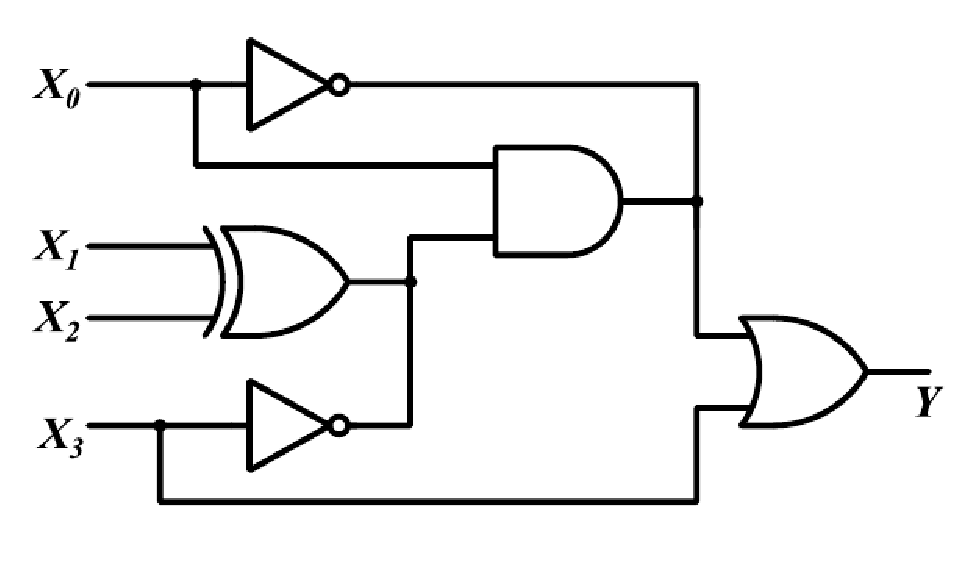
\includegraphics[width=\columnwidth]{./figs/47_gate_18.eps}
%\resizebox {\columnwidth} {!} {
%%\documentclass{standalone}
%\usepackage{tikz}
%\usetikzlibrary{matrix,calc}


%Empty Karnaugh map 4x4
\newenvironment{Karnaugh}%
{
\begin{tikzpicture}[baseline=(current bounding box.north),scale=0.8]
\draw (0,0) grid (4,4);
\draw (0,4) -- node [pos=0.7,above right,anchor=south west] {ab} node [pos=0.7,below left,anchor=north east] {cd} ++(135:1);
%
\matrix (mapa) [matrix of nodes,
        column sep={0.8cm,between origins},
        row sep={0.8cm,between origins},
        every node/.style={minimum size=0.3mm},
        anchor=8.center,
        ampersand replacement=\&] at (0.5,0.5)
{
                       \& |(c00)| 00         \& |(c01)| 01         \& |(c11)| 11         \& |(c10)| 10         \& |(cf)| \phantom{00} \\
|(r00)| 00             \& |(0)|  \phantom{0} \& |(1)|  \phantom{0} \& |(3)|  \phantom{0} \& |(2)|  \phantom{0} \&                     \\
|(r01)| 01             \& |(4)|  \phantom{0} \& |(5)|  \phantom{0} \& |(7)|  \phantom{0} \& |(6)|  \phantom{0} \&                     \\
|(r11)| 11             \& |(12)| \phantom{0} \& |(13)| \phantom{0} \& |(15)| \phantom{0} \& |(14)| \phantom{0} \&                     \\
|(r10)| 10             \& |(8)|  \phantom{0} \& |(9)|  \phantom{0} \& |(11)| \phantom{0} \& |(10)| \phantom{0} \&                     \\
|(rf) | \phantom{00}   \&                    \&                    \&                    \&                    \&                     \\
};
}%
{
\end{tikzpicture}
}


%Defines 8 or 16 values (0,1,X)
\newcommand{\contingut}[1]{%
\foreach \x [count=\xi from 0]  in {#1}
     \path (\xi) node {\x};
}



%\begin{document}
    \begin{Karnaugh}
        \contingut{1,x,1,x,x,,1,,1,,x,,,,,}
     
    \end{Karnaugh}
    %
  
    %
   
%\end{document}

%}
\caption{}
\label{fig:problem53}
\end{figure}

 \end{enumerate}

\end{document}
